\documentclass[11pt,a4paper]{article}
\usepackage[utf8]{inputenc}
\usepackage[T1]{fontenc}
\usepackage{amsmath,amssymb}
\usepackage{geometry}
\geometry{margin=2.4cm}
\usepackage{booktabs}
\usepackage{array}
\usepackage{tikz}
\usetikzlibrary{arrows.meta,positioning}

\newcommand{\ssc}[1]{\texttt{#1}}
\newcommand{\ud}{\mathrm{d}}

\title{Modello Simscape \ssc{mos\_dyn}\\
\large Dinamica di commutazione di un MOSFET di potenza}
\author{}
\date{Luglio 2026 --- rev.\ 1.0}

\begin{document}
\maketitle

\section{Scopo e limiti}

Il componente \ssc{mos\_dyn} riproduce la forma d'onda dei transitori di
accensione e spegnimento di un MOSFET di potenza (Si o SiC). È il
corrispettivo di \ssc{igbt\_dyn} e ha lo stesso ambito d'uso: double pulse
test, verifica del picco di sovratensione, del ringing e del reverse
recovery, dimensionamento di snubber e resistenze di gate.

\medskip
\noindent Cosa il modello risolve:
\begin{itemize}
  \item $\ud v/\ud t$ e $\ud i/\ud t$ reali, con plateau di Miller e la
        loro dipendenza da $R_g$, $V_{drv}$, $I_d$ e $V_{dc}$;
  \item conduzione del canale nei due quadranti, quindi rettificazione
        sincrona e comportamento in dead-time;
  \item reverse recovery del diodo di body con controllo di carica: $I_{rr}$
        e $t_{rr}$ emergono dal $\ud i/\ud t$ del circuito, non sono imposti;
  \item retroazione dell'induttanza di source comune sul loop di gate;
  \item clamp di valanga opzionale.
\end{itemize}

\noindent Cosa il modello non risolve:
\begin{itemize}
  \item perdite ed effetti termici: nessuna porta termica, nessun parametro
        dipendente da $T_j$. I parametri vanno estratti dalle curve alla
        temperatura di interesse (tipicamente $125\,^\circ$C o $150\,^\circ$C);
  \item degradazione della soglia, corto circuito, $\ud v/\ud t$ spurio da
        turn-on parassita (quest'ultimo in realtà emerge, se il circuito di
        gate esterno lo consente, perché $C_{gd}$ è modellata);
  \item effetti bidimensionali del canale (JFET region, saturazione della
        velocità) se non attraverso il fit di $K_p$;
  \item per i dispositivi SiC, la caratteristica di trasferimento reale è
        meno ``quadratica'' di quella di un MOSFET Si~\cite{McNutt2007,Mudholkar2014}:
        il fit va fatto
        vicino alla corrente nominale, non vicino alla soglia
        (sezione~\ref{sec:param}).
\end{itemize}

\section{Topologia interna}

\begin{center}
\begin{tikzpicture}[
  term/.style={circle,draw,inner sep=1.2pt,fill=black},
  box/.style={draw,rounded corners=1pt,inner sep=3pt,font=\footnotesize,align=center,fill=white},
  wire/.style={line width=0.6pt}]

% --- buses -------------------------------------------------------------
\draw[wire] (3,2.4) -- (8.6,2.4);
\draw[wire] (3,-2.4) -- (8.6,-2.4);

% --- terminals ---------------------------------------------------------
\node[term,label=left:{$G$}] (G) at (0,0) {};
\draw[wire] (0,0) -- (3,0);
\node[box] at (1.5,0) {$R_g$};
\node[term,label=above:{\footnotesize $g_i$}] at (3,0) {};

\node[term,label=above:{$D$}] at (6,4.2) {};
\draw[wire] (6,4.2) -- (6,2.4);
\node[box] at (6,3.3) {$R_d,\;L_d$};
\node[term,label={[shift={(0.45,-0.62)}]\footnotesize $d_i$}] at (6,2.4) {};

\node[term,label=below:{$S$}] at (6,-4.2) {};
\draw[wire] (6,-4.2) -- (6,-2.4);
\node[box] at (6,-3.3) {$L_s$};
\node[term,label={[shift={(0.45,-0.05)}]\footnotesize $s_i$}] at (6,-2.4) {};

% --- gate capacitances -------------------------------------------------
\draw[wire] (3,0) -- (3,2.4);
\node[box] at (3,1.4) {$C_{gd}(v_{gd})$};
\draw[wire] (3,0) -- (3,-2.4);
\node[box] at (3,-1.4) {$C_{gs}$};

% --- vertical branches -------------------------------------------------
\draw[wire] (5,2.4) -- (5,-2.4);
\node[box] at (5,0) {canale};
\draw[wire] (7.2,2.4) -- (7.2,-2.4);
\node[box] at (7.2,0) {$C_{ds}(v_{ds})$};
\draw[wire] (8.6,2.4) -- (8.6,-2.4);
\node[box] at (8.6,0) {diodo\\body\\(LM)};
\end{tikzpicture}
\end{center}

\noindent Tre terminali esterni ($G$, $D$, $S$) e tre nodi interni
($g_i$, $d_i$, $s_i$). Le variabili di stato sono $v_{gs}=v_{g_i}-v_{s_i}$,
$v_{gd}=v_{g_i}-v_{d_i}$, le correnti nei reofori $i_{dd}$, $i_{ss}$ e la
carica immagazzinata $q_M$ del diodo di body. Anche la tensione
drain-source interna $v_{ds}=v_{gs}-v_{gd}$ è dichiarata come variabile e
legata ai potenziali di nodo, pur essendo linearmente dipendente dalle altre
due: le tre capacità a delta danno tre equazioni differenziali, e Simscape
richiede che il numero di equazioni contenenti \ssc{der()} coincida con il
numero di variabili che vi compaiono. Scrivere invece
$i_{ds}=C_{ds}(\dot v_{gs}-\dot v_{gd})$ con $v_{ds}$ come
\emph{intermediate} produce l'errore \emph{``Total size of differential
equations does not match the total size of differential variables''} in fase
di compilazione della rete. La dipendenza fra i tre stati viene risolta dal
compilatore per riduzione d'indice.

\medskip
\noindent \textbf{Nota importante.} $C_{ds}$ \emph{è} la capacità di
deplezione della giunzione body-drain. Il blocco diodo contiene quindi solo
la carica di diffusione (modello Lauritzen--Ma) e nessuna capacità di
giunzione propria, altrimenti la carica capacitiva verrebbe contata due
volte. Questa è la differenza strutturale principale rispetto al
\ssc{diode\_rr} usato in esterno con \ssc{igbt\_dyn}, dove il diodo è un
dispositivo separato e la sua $C_j$ è sua.

\section{Canale MOS}

\subsection{Formulazione simmetrica}

Il canale di un MOSFET è fisicamente simmetrico: drain e source si scambiano
quando $v_{ds}$ cambia segno. La forma usata è la legge quadratica di
Shichman--Hodges~\cite{Shichman1968} riscritta in forma simmetrica
\begin{equation}
  i_{ch} = \frac{K_p}{2}\Big[\langle v_{gs}-V_{th}\rangle^2
                            -\langle v_{gd}-V_{th}\rangle^2\Big]
           \,\big(1+\lambda|v_{ds}|\big),
  \label{eq:chan}
\end{equation}
dove $\langle x\rangle$ è la parte positiva regolarizzata
\begin{equation}
  \langle x\rangle = \tfrac12\Big(x+\sqrt{x^2+V_{sm}^2}\Big).
\end{equation}

La~\eqref{eq:chan} contiene i tre regimi senza istruzioni condizionali:
\begin{itemize}
  \item \emph{saturazione diretta} ($v_{gd}<V_{th}$, cioè $v_{ds}>v_{gs}-V_{th}$):
        il secondo termine si annulla e
        $i_{ch}=\frac{K_p}{2}(v_{gs}-V_{th})^2$;
  \item \emph{triodo} ($v_{gd}>V_{th}$): sostituendo $v_{gd}=v_{gs}-v_{ds}$,
        \[
          i_{ch}=\frac{K_p}{2}\big[(v_{gs}-V_{th})^2-(v_{gs}-v_{ds}-V_{th})^2\big]
                =K_p\Big[(v_{gs}-V_{th})\,v_{ds}-\frac{v_{ds}^2}{2}\Big];
        \]
  \item \emph{terzo quadrante} ($v_{ds}<0$): $v_{gd}>v_{gs}$, il secondo
        termine domina e $i_{ch}<0$. Con il gate acceso il canale porta la
        corrente inversa (rettificazione sincrona) e il diodo di body resta
        quasi spento; in dead-time il canale si chiude e la corrente passa
        nel diodo. È il meccanismo che determina quanta carica $Q_{rr}$ viene
        effettivamente immagazzinata, e quindi quanto è grande il picco di
        recovery del turn-on successivo.
\end{itemize}

L'assenza di condizionali evita zero-crossing e mode chart: il solver vede
una funzione $C^\infty$.

\subsection{Resistenza di conduzione}

In triodo, per $v_{ds}\to 0$,
\begin{equation}
  R_{ch}=\frac{1}{K_p\,(V_{gs,on}-V_{th})},
  \qquad
  R_{ds(on)}=R_{ch}+R_d .
\end{equation}
$R_d$ rappresenta la resistenza di drift (e di package) ed è il parametro
con cui si aggiusta $R_{ds(on)}$ a valore di datasheet una volta fissati
$V_{th}$ e $K_p$ dalla caratteristica di trasferimento. Tenerli separati è
importante: $K_p$ governa la dinamica (plateau di Miller, $\ud i/\ud t$),
$R_d$ governa solo la statica.

\subsection{Plateau di Miller e $\ud v/\ud t$}

Durante la commutazione la corrente di drain è imposta dal carico
induttivo, quindi il gate si ferma alla tensione di plateau
\begin{equation}
  V_{pl}=V_{th}+\sqrt{\frac{2 I_d}{K_p}} .
  \label{eq:vpl}
\end{equation}
Tutta la corrente di gate si scarica su $C_{gd}$ e la pendenza di tensione è
\begin{equation}
  \frac{\ud v_{ds}}{\ud t}\simeq
  \frac{V_{drv}-V_{pl}}{\big(R_{g,ext}+R_g\big)\,C_{gd}(v_{ds})} .
  \label{eq:dvdt}
\end{equation}
Poiché $C_{gd}$ varia di due o tre decadi lungo l'escursione di tensione, il
$\ud v/\ud t$ non è costante: è lento vicino a zero volt e rapidissimo ad
alta tensione (o viceversa allo spegnimento). Questo è il motivo per cui una
$C_{gd}$ costante non è utilizzabile per lo studio degli snubber, ed è la
ragione della~\eqref{eq:cgd}.

\subsection{$\ud i/\ud t$ e induttanza di source comune}

Nella fase di salita della corrente il canale è in saturazione; con
$g_m=K_p(v_{gs}-V_{th})=\sqrt{2K_pI_d}$ e maglia di gate
$v_{drv}=R_{g,tot}\,i_g+v_{gs}+L_s\,\ud i_d/\ud t$ si ottiene
\begin{equation}
  \frac{\ud i_d}{\ud t}\simeq
  \frac{g_m\,\big(V_{drv}-V_{pl}\big)}{R_{g,tot}\,C_{iss}+g_m L_s}.
  \label{eq:didt}
\end{equation}
Il termine $g_mL_s$ al denominatore è la retroazione negativa
dell'induttanza di source comune: con $g_m$ elevato (SiC) bastano pochi nH
per dimezzare il $\ud i/\ud t$. Nel modello questo effetto non è imposto ma
emerge, perché il loop di gate è riferito al nodo interno $s_i$ mentre la
corrente di potenza attraversa $L_s$. Se il dispositivo reale ha un Kelvin
source, si imposti $L_s$ al solo valore condiviso (tipicamente
$1\div3$~nH) e si porti il resto nell'induttanza di loop esterna.

\section{Capacità non lineari}

\begin{align}
  C_{gd}(v_{gd}) &= \frac{C_{gd0}}{\big(1+\langle v_{gd}\rangle/V_{jg}\big)^{m_g}},
  \label{eq:cgd}\\[2mm]
  C_{ds}(v_{ds}) &= \frac{C_{ds0}}{\big(1+\langle v_{ds}\rangle/V_{jd}\big)^{m_d}},
  \qquad C_{gs}=\text{cost.}
\end{align}
La parte positiva $\langle\cdot\rangle$ agisce da clamp: per polarizzazione
negativa la giunzione è in accumulazione e la capacità satura al valore di
ossido $C_{gd0}$, invece di divergere come farebbe la legge di deplezione
pura per $v\to -V_j$. È lo stesso accorgimento usato in \ssc{igbt\_dyn}.

Le correnti di spostamento sono scritte in forma $C(v)\,\ud v/\ud t$:
\begin{equation}
  i_{gs}=C_{gs}\dot v_{gs},\qquad
  i_{gd}=C_{gd}(v_{gd})\,\dot v_{gd},\qquad
  i_{ds}=C_{ds}(v_{ds})\,\big(\dot v_{gs}-\dot v_{gd}\big).
\end{equation}
L'ultima espressione evita di dichiarare $v_{ds}$ come stato: la sua
derivata è ricostruita dagli altri due.

\subsection{Carica ed energia di uscita}

Con la legge di deplezione, ponendo $u=V/V_j$, si ottengono in forma chiusa
\begin{align}
  Q_{oss}(V)&=\frac{C_0 V_j}{1-m}\Big[(1+u)^{1-m}-1\Big], \\
  E_{oss}(V)&=C_0V_j^2\left\{\frac{(1+u)^{2-m}-1}{2-m}-\frac{(1+u)^{1-m}-1}{1-m}\right\},
  \qquad m\neq 1,2 .
\end{align}
Sono le due grandezze da confrontare con le curve $Q_{oss}(V_{ds})$ e
$E_{oss}(V_{ds})$ del datasheet per validare il fit di $C_{ds0}$, $V_{jd}$,
$m_d$. Per i SiC la quasi totalità della ``carica di recovery'' misurata è in
realtà $Q_{oss}$, non carica di diffusione: se il fit di $E_{oss}$ è corretto,
l'energia di turn-on nel double pulse test viene giusta quasi
indipendentemente dai parametri del diodo di body.

\medskip
\noindent Due avvertenze sulle curve di datasheet. La $C_{oss}$ misurata con
impedenzimetro a piccolo segnale non coincide con quella vista in commutazione:
nei superjunction si osserva un'isteresi di $C_{oss}$ che rende $E_{oss}$ di
datasheet ottimistico~\cite{Fedison2014,Fedison2016,Roig2015}. Il modello qui
usato è privo di isteresi (la carica è funzione univoca della tensione), quindi
riproduce la traiettoria di tensione ma non la dissipazione associata; per lo
studio di snubber e sovratensioni questo non è un limite, per il calcolo delle
perdite in soft switching lo è.

\section{Diodo di body}

\subsection{Modello a controllo di carica}

Il diodo intrinseco usa il modello a due cariche di
Lauritzen--Ma~\cite{Lauritzen1991,Ma1997}, derivato dal concetto di carica
concentrata di Linvill~\cite{Linvill1958}; per una rassegna dei modelli di
diodo di potenza si veda~\cite{Tan1999}:
$q_E$ è la carica al bordo della giunzione (istantanea, legata alla
tensione) e $q_M$ è la carica totale immagazzinata (stato dinamico).
\begin{align}
  q_E &= I_s\,\tau\left(e^{v_j/(NV_T)}-1\right), \label{eq:qE}\\
  i   &= \frac{q_E-q_M}{T_M} + G_{off}\,v_j, \label{eq:ilm}\\
  \frac{\ud q_M}{\ud t} &= \frac{q_E-q_M}{T_M}-\frac{q_M}{\tau},
  \label{eq:qM}
\end{align}
con $v_j=-v_{ds}-R_{sd}\,i$.

In conduzione stazionaria $\dot q_M=0$ dà $q_M=q_E\,\tau/(\tau+T_M)$ e
quindi la caratteristica statica
\begin{equation}
  I_F=\frac{I_s\,\tau}{\tau+T_M}\left(e^{V_F/(NV_T)}-1\right)+\ldots,
  \qquad V_{AK}=V_F+R_{sd}I_F .
\end{equation}
Allo spegnimento la~\eqref{eq:qM} impedisce a $q_M$ di annullarsi
istantaneamente: la corrente continua a scorrere in inverso finché la carica
non è stata estratta, ed è questo che genera $I_{rr}$ e la coda. Nulla è
imposto a priori: la profondità del picco dipende dal $\ud i/\ud t$ che il
circuito esterno (induttanza di loop, $R_g$ del transistor che commuta)
riesce a produrre.

\subsection{Estrazione dei parametri di carica}

Dai dati di datasheet $Q_{rr}$ e $I_{rr}$ misurati a $\ud i/\ud t=a$:
\begin{align}
  t_{tail}&=\frac{Q_{rr}}{I_{rr}}-\frac{I_{rr}}{2a}, &
  \tau &= t_{tail}+\frac{I_{rr}}{a}, &
  T_M &= \frac{\tau\,t_{tail}\,a}{I_{rr}} .
  \label{eq:extract}
\end{align}
Condizione di consistenza: il modello a due cariche ha solo due gradi di
libertà, quindi non ogni terna $(Q_{rr},I_{rr},a)$ è rappresentabile. Perché
risulti $T_M<\tau$ (diodo con buon rapporto conduzione/immagazzinamento)
occorre
\begin{equation}
  I_{rr}>\sqrt{\tfrac{2}{3}\,a\,Q_{rr}} .
\end{equation}
Se il datasheet dà una coppia che viola la condizione, il fit va rifatto su
un punto $\ud i/\ud t$ diverso, oppure si accetta un errore su $I_{rr}$
(tipicamente il modello sottostima il picco del $10\div20\%$, come già
osservato sul modello di tiristore).

\subsection{Regolarizzazione dell'esponenziale}

L'esponenziale della~\eqref{eq:qE} è sostituita da una versione linearizzata
sopra $V_{lin}$, senza istruzioni condizionali:
\begin{equation}
  x=\frac{v_j}{NV_T},\quad
  x_l=\frac{V_{lin}}{NV_T},\quad
  x_s=x_l-\tfrac12\Big[(x_l-x)+\sqrt{(x_l-x)^2+\epsilon^2}\Big],\quad
  e_x=e^{x_s}\big(1+x-x_s\big).
\end{equation}
$x_s$ è un $\min(x,x_l)$ regolarizzato: sotto soglia $x_s\simeq x$ e
$e_x\simeq e^x$; sopra soglia $x_s\simeq x_l$ e $e_x$ prosegue linearmente
con la stessa derivata. Si evita l'overflow senza introdurre eventi.
$V_{lin}$ va posto sopra il ginocchio del diodo: $\sim0{,}8$~V per il Si,
$\sim3{,}5$~V per il SiC.

$G_{off}$ è una conduttanza di dispersione ($10^{-9}$~S) che migliora il
condizionamento della matrice in blocking; non ha significato fisico.

\section{Clamp di valanga}

\begin{equation}
  i_{av}=G_{av}\,\big\langle v_{ds}-BV\big\rangle
\end{equation}
Sopra $BV$ il dispositivo diventa una sorgente di corrente con pendenza
$G_{av}$; sotto, la corrente è nulla a meno del residuo di
regolarizzazione. Serve quando si vuole valutare l'energia di valanga in
commutazione non clampata, o semplicemente per impedire che una simulazione
diverga in caso di overshoot patologico. Il valore di default
($BV=10^5$~V) lo disattiva: va impostato al $V_{(BR)DSS}$ di datasheet solo
se lo si vuole attivo, altrimenti il picco di sovratensione reale verrebbe
tosato senza avvisare.

\section{Parametrizzazione}\label{sec:param}

\subsection{Procedura}

\begin{enumerate}
  \item $V_{th}$, $K_p$: due punti sulla caratteristica di trasferimento
        $I_d(V_{gs})$ a caldo, presi \emph{attorno alla corrente nominale}
        (per il SiC il fit vicino alla soglia dà un $K_p$ troppo piccolo e un
        plateau di Miller sbagliato). Verifica incrociata: il $V_{pl}$
        della~\eqref{eq:vpl} deve corrispondere al plateau della curva di
        gate charge del datasheet.
  \item $R_d=R_{ds(on)}-1/[K_p(V_{gs,on}-V_{th})]$. Se viene negativo,
        $K_p$ è troppo basso: rifare il punto~1.
  \item $C_{gs}=C_{iss}-C_{rss}$ letti ad alta tensione (dove $C_{rss}$ è
        trascurabile, $C_{gs}\simeq C_{iss}$).
  \item $C_{gd0}$, $V_{jg}$, $m_g$: fit di $C_{rss}(V_{ds})$ in scala
        log-log. $C_{gd0}$ è il valore a $V_{ds}\to0$.
  \item $C_{ds0}$, $V_{jd}$, $m_d$: fit di $C_{oss}-C_{rss}$; verifica su
        $E_{oss}$ e $Q_{oss}$.
  \item $I_s$, $N$, $R_{sd}$: dalla curva $I_F(V_F)$ del diodo di body a
        caldo.
  \item $\tau$, $T_M$: dalle~\eqref{eq:extract}.
  \item $L_d$, $L_s$, $R_g$: da datasheet del package (o
        $L_d\simeq10$~nH, $L_s\simeq5$~nH per un modulo, molto meno per un
        discreto con Kelvin).
\end{enumerate}

\subsection{Due set di riferimento}

\begin{center}
\begin{tabular}{llrrl}
\toprule
Parametro & Descrizione & SiC $1200$~V & Si SJ $650$~V & Unità \\
\midrule
\ssc{Vth}  & tensione di soglia            & $5{,}0$   & $4{,}0$   & V \\
\ssc{Kp}   & transconduttanza              & $30$      & $15$      & A/V$^2$ \\
\ssc{lam}  & modulazione di canale         & $0$       & $0$       & 1/V \\
\ssc{Rd}   & resistenza di drift           & $2{,}0$   & $20$      & m$\Omega$ \\
\ssc{Rg}   & gate interno                  & $1{,}0$   & $2{,}0$   & $\Omega$ \\
\ssc{Ld}   & induttanza di drain           & $10$      & $5$       & nH \\
\ssc{Ls}   & source comune                 & $5$       & $3$       & nH \\
\midrule
\ssc{Cgs}  & $C_{iss}-C_{rss}$             & $20$      & $5{,}0$   & nF \\
\ssc{Cgd0} & Miller a $0$~V                & $6{,}0$   & $3{,}0$   & nF \\
\ssc{Vjg}  & potenziale di giunzione       & $5{,}0$   & $1{,}0$   & V \\
\ssc{mg}   & coefficiente di grading       & $1{,}5$   & $2{,}5$   & --- \\
\ssc{Cds0} & $C_{oss}-C_{rss}$ a $0$~V     & $40$      & $8{,}0$   & nF \\
\ssc{Vjd}  & potenziale di giunzione       & $8{,}0$   & $1{,}0$   & V \\
\ssc{md}   & coefficiente di grading       & $0{,}5$   & $2{,}2$   & --- \\
\midrule
\ssc{Is}   & corrente di saturazione       & $10^{-14}$& $10^{-12}$& A \\
\ssc{N}    & coefficiente di emissione     & $2{,}5$   & $2{,}0$   & --- \\
\ssc{Rsd}  & serie del diodo               & $2{,}5$   & $25$      & m$\Omega$ \\
\ssc{taud} & vita media $\tau$             & $17$      & $114$     & ns \\
\ssc{TM}   & tempo di transito $T_M$       & $3{,}2$   & $36$      & ns \\
\ssc{Vlin} & linearizzazione esponenziale  & $3{,}5$   & $0{,}8$   & V \\
\midrule
\ssc{BV}   & valanga (disattivata)         & $10^{5}$  & $10^{5}$  & V \\
\ssc{Vsm}  & tensione di smoothing         & $50$      & $50$      & mV \\
\bottomrule
\end{tabular}
\end{center}

\noindent Il set SiC corrisponde a un modulo da $\sim\!300$~A,
$R_{ds(on)}\simeq4{,}2$~m$\Omega$, con
$\tau,T_M$ ricavati da $Q_{rr}=2\,\mu$C e $I_{rr}=120$~A a
$5$~kA/$\mu$s. Il set Si superjunction corrisponde a
$Q_{rr}=8\,\mu$C, $I_{rr}=70$~A a $500$~A/$\mu$s. Si noti la differenza dei
coefficienti di grading: il collasso brusco di $C_{oss}$ tipico del
superjunction richiede $m_d>2$, mentre il SiC ha un andamento molto più
regolare.

\section{Uso nel double pulse test}

\subsection{Schema}

\begin{center}
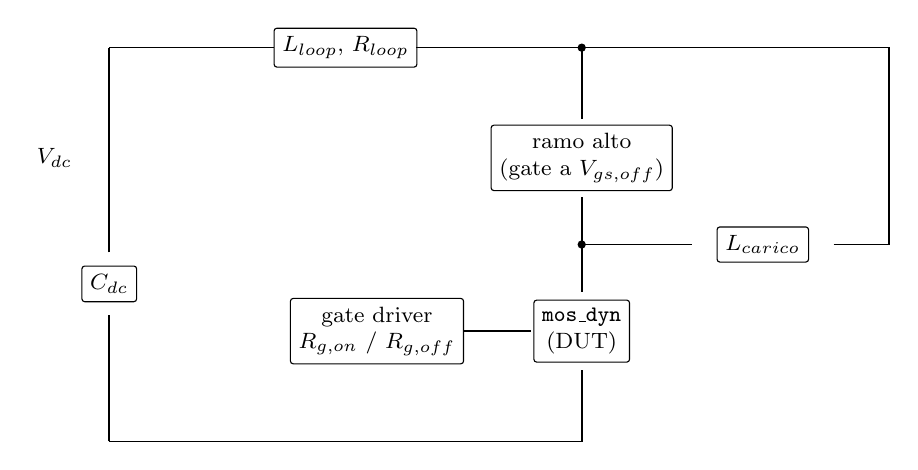
\begin{tikzpicture}[
  lbl/.style={font=\footnotesize},
  box/.style={draw,rounded corners=1pt,inner sep=3pt,font=\footnotesize,align=center,fill=white},
  wire/.style={line width=0.6pt}]

% --- DC bus -----------------------------------------------------------
\draw[wire] (0,0) -- (0,1.6);
\draw[wire] (0,2.4) -- (0,5);
\node[box] at (0,2.0) {$C_{dc}$};
\node[lbl,left] at (-0.35,3.6) {$V_{dc}$};

% --- top rail with loop inductance ------------------------------------
\draw[wire] (0,5) -- (2.1,5);
\node[box] at (3.0,5) {$L_{loop},\,R_{loop}$};
\draw[wire] (3.9,5) -- (6,5);

% --- high side --------------------------------------------------------
\draw[wire] (6,5) -- (6,4.1);
\node[box] at (6,3.6) {ramo alto\\(gate a $V_{gs,off}$)};
\draw[wire] (6,3.1) -- (6,2.5);

% --- midpoint and load ------------------------------------------------
\fill (6,2.5) circle (1.5pt);
\draw[wire] (6,2.5) -- (7.4,2.5);
\node[box] at (8.3,2.5) {$L_{carico}$};
\draw[wire] (9.2,2.5) -- (9.9,2.5) -- (9.9,5) -- (6,5);
\fill (6,5) circle (1.5pt);

% --- DUT --------------------------------------------------------------
\draw[wire] (6,2.5) -- (6,1.9);
\node[box] at (6,1.4) {\ssc{mos\_dyn}\\(DUT)};
\draw[wire] (6,0.9) -- (6,0) -- (0,0);

% --- gate driver ------------------------------------------------------
\node[box] at (3.4,1.4) {gate driver\\$R_{g,on}$ / $R_{g,off}$};
\draw[wire] (4.5,1.4) -- (5.35,1.4);
\end{tikzpicture}
\end{center}

Per le regole pratiche di layout, di misura e di allineamento $v$--$i$ nel
double pulse test si vedano~\cite{Zhang2017,Levett2020}.

Il DUT basso è \ssc{mos\_dyn}; il ramo alto può essere un secondo
\ssc{mos\_dyn} con gate tenuto a $V_{gs,off}$ (così il recovery avviene sul
diodo di body, che è il caso reale in un half-bridge) oppure un diodo esterno
se si sta caratterizzando una configurazione con SBD antiparallelo.

\subsection{Cosa impostare}

\begin{center}
\begin{tabular}{ll}
\toprule
Elemento & Nota \\
\midrule
$C_{dc}$      & grande ($\ge100\,\mu$F) più un condensatore di snubber locale, se presente \\
$L_{loop}$    & induttanza di maglia di commutazione, il parametro che governa l'overshoot \\
              & (tipicamente $10\div40$~nH per un modulo con bus laminato) \\
$R_{loop}$    & resistenza serie di maglia, $1\div10$~m$\Omega$: senza di essa il ringing \\
              & non si smorza mai ed è irrealistico \\
$L_{carico}$  & induttanza d'aria, tale da avere $\ud i/\ud t$ contenuto durante i due impulsi \\
Gate driver   & sorgente di tensione con $R_{g,on}$, $R_{g,off}$ separati (diodo di by-pass) \\
              & e livelli reali: $+15/-4$~V per SiC, $+15/0$ o $-5$~V per Si \\
\bottomrule
\end{tabular}
\end{center}

Il picco di sovratensione allo spegnimento è
$V_{pk}\simeq V_{dc}+L_{loop}\,\ud i/\ud t$ con $\ud i/\ud t$ dato
dalla~\eqref{eq:didt}: se il valore simulato non torna con la misura, il
problema è quasi sempre $L_{loop}$ o $K_p$, non il modello del diodo.

\subsection{Grandezze da estrarre}

$I_{rr}$ e $Q_{rr}$ effettivi (integrale della corrente inversa del ramo
alto), $\ud v/\ud t$ e $\ud i/\ud t$ al $10\div90\%$, $V_{pk}$ allo
spegnimento, frequenza e smorzamento del ringing, energia dissipata
$\int v\,i\,\ud t$ sul dispositivo (che qui è un risultato, non un
parametro: è un buon controllo incrociato contro l'$E_{on}/E_{off}$ di
datasheet).

\section{Dimensionamento dello snubber}

Il dimensionamento classico degli snubber RC e RCD è trattato
in~\cite{McMurray1972,Mohan2003}. Per uno snubber RC ai capi del
dispositivo, partendo da un valore di
capacità pari a qualche volta la $C_{oss}$ equivalente alla tensione di
lavoro:
\begin{equation}
  C_s \simeq (3\div5)\,C_{oss,eq},
  \qquad
  R_s=\sqrt{\frac{L_{loop}}{C_s}},
  \qquad
  P_s = C_s V_{dc}^2 f_{sw}.
\end{equation}
$R_s$ così scelta smorza criticamente la maglia $L_{loop}$--$C_s$; la
potenza dissipata $P_s$ è indipendente da $R_s$ ed è quasi sempre il vincolo
progettuale reale. Con il modello si verifica l'efficacia direttamente:
si confrontano $V_{pk}$ e l'ampiezza del ringing con e senza snubber, e si
controlla di quanto peggiorano $\ud v/\ud t$ ed $E_{off}$.

Alternativa da valutare con lo stesso modello: aumentare $R_{g,off}$ (costa
energia di commutazione ma niente componenti), oppure ridurre $L_{loop}$
(sempre la soluzione migliore, quando è possibile).

\section{Differenze rispetto a \ssc{igbt\_dyn}}

\begin{center}
\begin{tabular}{lll}
\toprule
& \ssc{igbt\_dyn} & \ssc{mos\_dyn} \\
\midrule
Corrente di coda & presente ($f_{tail}$, $\tau_T$) & assente \\
Conduzione inversa & nessuna & canale simmetrico \\
Diodo antiparallelo & esterno (\ssc{diode\_rr}) & intrinseco (body) \\
Capacità di giunzione del diodo & nel \ssc{diode\_rr} & è $C_{ds}$ \\
Caduta in conduzione & $V_{ce,sat}$, offset & resistiva, $R_{ds(on)}$ \\
Parassiti di package & esterni & $R_d,L_d,L_s$ interni \\
\bottomrule
\end{tabular}
\end{center}

Per un modello IGBT fisico completo, in cui la coda deriva dalla ricombinazione
nella regione di drift invece che da un decadimento esponenziale imposto,
si veda~\cite{Hefner1994}.

L'assenza della corrente di coda elimina anche l'equazione di stato $q_T$
che aveva dato problemi di convergenza in \ssc{igbt\_dyn}: il modello
MOSFET ha uno stato dinamico in meno per dispositivo e in genere converge
meglio.

\section{Note numeriche}

\begin{itemize}
  \item Sintassi, sezioni \ssc{intermediates} e regole di dichiarazione delle
        variabili: \cite{MathWorksSSC}.
  \item Solver: \ssc{daessc} con \ssc{ode23t}, oppure \ssc{ode15s}. Passo
        massimo dell'ordine di $1$~ns per un DPT di qualche decina di~$\mu$s;
        \ssc{RelTol}~$10^{-5}$, \ssc{AbsTol} automatico.
  \item Simscape: local solver disattivato, \ssc{Constraint residual
        tolerance} lasciata al default. Se compaiono errori di algebra
        lineare, la causa più comune è un nodo senza percorso a massa in
        continua: aggiungere una resistenza di leakage elevata
        ($10^{6}\,\Omega$) in parallelo al bus.
  \item $V_{sm}$ regola tutte le regolarizzazioni. Aumentarlo
        ($100\div200$~mV) se il solver fatica; il prezzo è una piccola
        corrente residua sotto soglia e un ginocchio più morbido.
  \item L'induttanza $L_s$ non va posta esattamente a zero: si usi almeno
        $0{,}1$~nH per non degenerare il ramo in un vincolo algebrico.
  \item Inizializzazione: con il gate a $V_{gs,off}$ e il bus carico, il
        modello parte in blocking senza problemi; se si vuole partire con il
        dispositivo acceso, si dia una priorità alta a $v_{gs}$.
\end{itemize}

\section{Riepilogo delle equazioni}

\begin{align*}
  v_{gs}&=v_{g_i}-v_{s_i}, \qquad v_{gd}=v_{g_i}-v_{d_i}, \qquad v_{ds}=v_{gs}-v_{gd}\\
  v_G-v_{g_i}&=R_g i_g\\
  v_D-v_{d_i}&=R_d i_{dd}+L_d \dot i_{dd}\\
  v_{s_i}-v_S&=L_s \dot i_{ss}\\
  i_{ch}&=\tfrac{K_p}{2}\big[\langle v_{gs}-V_{th}\rangle^2-\langle v_{gd}-V_{th}\rangle^2\big](1+\lambda|v_{ds}|)\\
  i_{gs}&=C_{gs}\dot v_{gs}, \quad
  i_{gd}=C_{gd}(v_{gd})\dot v_{gd}, \quad
  i_{ds}=C_{ds}(v_{ds})(\dot v_{gs}-\dot v_{gd})\\
  q_E&=I_s\tau\,(e_x-1), \quad
  i_{bd}=\frac{q_E-q_M}{T_M}+G_{off}v_j, \quad
  \dot q_M=\frac{q_E-q_M}{T_M}-\frac{q_M}{\tau}\\
  i_{av}&=G_{av}\langle v_{ds}-BV\rangle
\end{align*}


\begin{thebibliography}{99}

\bibitem{Linvill1958} J.~G.~Linvill, ``Lumped models of transistors and
diodes,'' \emph{Proc. IRE}, vol.~46, no.~6, pp.~1141--1152, Jun.~1958.

\bibitem{Shichman1968} H.~Shichman and D.~A.~Hodges, ``Modeling and simulation
of insulated-gate field-effect transistor switching circuits,''
\emph{IEEE J. Solid-State Circuits}, vol.~SC-3, no.~3, pp.~285--289, Sep.~1968.

\bibitem{McMurray1972} W.~McMurray, ``Optimum snubbers for power
semiconductors,'' \emph{IEEE Trans. Ind. Appl.}, vol.~IA-8, no.~5,
pp.~593--600, Sep.~1972.

\bibitem{Lauritzen1991} P.~O.~Lauritzen and C.~L.~Ma, ``A simple diode model
with reverse recovery,'' \emph{IEEE Trans. Power Electron.}, vol.~6, no.~2,
pp.~188--191, Apr.~1991. DOI: 10.1109/63.76804.

\bibitem{Hefner1994} A.~R.~Hefner and D.~M.~Diebolt, ``An experimentally
verified IGBT model implemented in the Saber circuit simulator,''
\emph{IEEE Trans. Power Electron.}, vol.~9, no.~5, pp.~532--542, Sep.~1994.

\bibitem{Ma1997} C.~L.~Ma, P.~O.~Lauritzen, and J.~Sigg, ``Modeling of power
diodes with the lumped-charge modeling technique,'' \emph{IEEE Trans. Power
Electron.}, vol.~12, no.~3, 1997.

\bibitem{Tan1999} C.~M.~Tan and K.~J.~Tseng, ``Using power diode models for
circuit simulations --- a comprehensive review,'' \emph{IEEE Trans. Ind.
Electron.}, vol.~46, no.~3, pp.~637--645, Jun.~1999.

\bibitem{Mohan2003} N.~Mohan, T.~M.~Undeland, and W.~P.~Robbins, \emph{Power
Electronics: Converters, Applications and Design}, 3rd~ed. Hoboken, NJ: Wiley,
2003, cap.~27 (snubber circuits).

\bibitem{McNutt2007} T.~R.~McNutt, A.~R.~Hefner, H.~A.~Mantooth, D.~Berning,
and S.-H.~Ryu, ``Silicon carbide power MOSFET model and parameter extraction
sequence,'' \emph{IEEE Trans. Power Electron.}, vol.~22, no.~2, pp.~353--363,
Mar.~2007.

\bibitem{Mudholkar2014} M.~Mudholkar, S.~Ahmed, M.~N.~Ericson, S.~S.~Frank,
C.~L.~Britton, and H.~A.~Mantooth, ``Datasheet driven silicon carbide power
MOSFET model,'' \emph{IEEE Trans. Power Electron.}, vol.~29, no.~5,
pp.~2220--2228, May~2014. DOI: 10.1109/TPEL.2013.2295774.

\bibitem{Fedison2014} J.~B.~Fedison, M.~Fornage, M.~J.~Harrison, and
D.~R.~Zimmanck, ``$C_{oss}$ related energy loss in power MOSFETs used in
zero-voltage-switched applications,'' in \emph{Proc. IEEE APEC}, 2014,
pp.~150--156.

\bibitem{Roig2015} J.~Roig and F.~Bauwens, ``Origin of anomalous $C_{oss}$
hysteresis in resonant converters with superjunction FETs,'' \emph{IEEE Trans.
Electron Devices}, vol.~62, no.~9, pp.~3092--3094, Sep.~2015.

\bibitem{Fedison2016} J.~B.~Fedison and M.~J.~Harrison, ``$C_{oss}$ hysteresis
in advanced superjunction MOSFETs,'' in \emph{Proc. IEEE APEC}, 2016,
pp.~247--252.

\bibitem{Zhang2017} Z.~Zhang, B.~Guo, F.~F.~Wang, E.~A.~Jones, L.~M.~Tolbert,
and B.~J.~Blalock, ``Methodology for wide band-gap device dynamic
characterization,'' \emph{IEEE Trans. Power Electron.}, vol.~32, no.~12,
pp.~9307--9318, Dec.~2017. DOI: 10.1109/TPEL.2017.2655491.

\bibitem{Baliga2019} B.~J.~Baliga, \emph{Fundamentals of Power Semiconductor
Devices}, 2nd~ed. Cham: Springer, 2019.

\bibitem{Levett2020} D.~Levett, Z.~Zheng, and T.~Frank, ``Double pulse testing:
the how, what and why,'' \emph{Bodo's Power Systems}, Apr.~2020.

\bibitem{Erickson2020} R.~W.~Erickson and D.~Maksimovi\'c, \emph{Fundamentals
of Power Electronics}, 3rd~ed. Cham: Springer, 2020.

\bibitem{MathWorksSSC} The MathWorks, Inc., \emph{Simscape Language Guide},
Natick, MA, USA.

\end{thebibliography}

\end{document}
